\documentclass[11pt,a4paper]{article}

% ─── Packages ────────────────────────────────────────────
\usepackage[T1]{fontenc}
\usepackage[utf8]{inputenc}
\usepackage[margin=2.5cm]{geometry}
\usepackage{setspace}\setstretch{1.15}
\usepackage{booktabs}
\usepackage{longtable}
\usepackage{tabularx}
\usepackage{graphicx}
\usepackage{float}
\usepackage{caption}
\usepackage{subcaption}
\usepackage{hyperref}
\usepackage{xcolor}
\usepackage{fancyhdr}
\usepackage{amsmath}
\usepackage{textcomp}
\usepackage{enumitem}
\usepackage{tcolorbox}
\tcbuselibrary{skins,breakable}
\usepackage{listings}
\usepackage{parskip}

% ─── Colors ──────────────────────────────────────────────
\definecolor{darkblue}{RGB}{26,58,92}
\definecolor{medblue}{RGB}{44,95,138}
\definecolor{lightblue}{RGB}{232,240,248}
\definecolor{algobg}{RGB}{245,248,252}
\definecolor{algoborder}{RGB}{70,130,180}
\definecolor{stepbg}{RGB}{252,250,245}
\definecolor{stepborder}{RGB}{180,160,100}
\definecolor{codegray}{RGB}{245,245,245}
\definecolor{codetext}{RGB}{40,40,40}
\definecolor{accent}{RGB}{192,57,43}

% ─── Hyperlinks ──────────────────────────────────────────
\hypersetup{colorlinks=true, linkcolor=darkblue, urlcolor=medblue, citecolor=darkblue, breaklinks=true}
\usepackage{xurl}

% ─── Headers ─────────────────────────────────────────────
\pagestyle{fancy}
\fancyhead[L]{\small\textit{MSc Computer Science --- Dissertation}}
\fancyhead[R]{\small\textit{Vision-Based Robotic Affordance Detection}}
\fancyfoot[C]{\thepage}
\renewcommand{\headrulewidth}{0.4pt}

% ─── Algorithm Box Style ─────────────────────────────────
\newtcolorbox{algorithmbox}[1][]{
  colback=algobg, colframe=algoborder,
  fonttitle=\bfseries, title=#1,
  arc=3pt, boxrule=0.8pt,
  left=8pt, right=8pt, top=4pt, bottom=4pt,
  before skip=8pt, after skip=8pt
}

% ─── Step Box Style ──────────────────────────────────────
\newtcolorbox{stepbox}[1][]{
  colback=stepbg, colframe=stepborder,
  fonttitle=\bfseries\sffamily, title=#1,
  arc=2pt, boxrule=0.6pt,
  left=8pt, right=8pt, top=3pt, bottom=3pt,
  before skip=6pt, after skip=6pt
}

% ─── Code listing style ─────────────────────────────────
\lstset{
  basicstyle=\small\ttfamily\color{codetext},
  backgroundcolor=\color{codegray},
  breaklines=true, frame=none,
  xleftmargin=4pt, xrightmargin=4pt,
  aboveskip=0pt, belowskip=0pt,
  columns=fullflexible
}

% ─── Tight list ──────────────────────────────────────────
\providecommand{\tightlist}{\setlength{\itemsep}{2pt}\setlength{\parskip}{0pt}}

% ═══════════════════════════════════════════════════════════
\begin{document}

% ─── TITLE PAGE ──────────────────────────────────────────
\begin{titlepage}
\centering
\vspace*{4cm}
{\Huge\bfseries\color{darkblue} Vision-Based Robotic Affordance\\[6pt]Detection and Feature Identification\par}
\vspace{1.2cm}
{\Large\itshape\color{medblue} A Simulation-Driven Approach to Bridging Perception and Manipulation\par}
\vspace{3cm}
{\large Degree: Master of Computer Science (MCS)\par}
\vspace{0.3cm}
{\large Project Type: Computer Vision \& Robotics Simulation\par}
\vfill
\end{titlepage}

% ─── TABLE OF CONTENTS ───────────────────────────────────
\tableofcontents
\newpage

% ═══════════════════════════════════════════════════════════
% ABSTRACT
% ═══════════════════════════════════════════════════════════
\section*{Abstract}
\addcontentsline{toc}{section}{Abstract}

\textbf{Autonomous robotic manipulation in unstructured environments requires perception systems that can identify not just what objects are present, but where and how a robot can physically interact with them --- a capability that remains challenging due to the gap between object-level recognition and feature-level geometric understanding.}

This dissertation presents a vision-based system for detecting manipulation-relevant geometric features --- apertures, planar surfaces, and protrusions --- on tabletop objects and mapping them to 3D world coordinates. The system uses exclusively classical computer vision algorithms (Hough Circle Transform, contour analysis, Canny Edge Detection) operating on synthetic RGB-D data generated through programmatic scene rendering, requiring no training data, no GPU hardware, and no deep learning infrastructure. Detected features are projected from 2D pixel coordinates into 3D world positions using camera intrinsic and extrinsic matrix transformations.

Quantitative evaluation across 300+ randomised trials demonstrates 80\% hole detection accuracy with 36mm mean 3D precision, 58\% surface detection with 6.2-pixel localisation error, and real-time performance at approximately 50ms per frame on CPU. Handle detection achieved only 10\%, identifying a clear limitation boundary where classical methods give way to learned approaches. Robustness testing across 12 orientations, 8 camera distances, and 20 multi-object clutter scenarios characterises the system's operational envelope. A 53-test automated suite achieves 100\% pass rate.

\textbf{The system's real-time performance (\textasciitilde50ms per frame on CPU) and lightweight architecture --- requiring no GPU, no training data, and no deep learning infrastructure --- make it readily deployable on resource-constrained robotic platforms such as embedded systems and edge devices. This positions the approach as a practical, low-cost perception module that can be directly integrated into existing robotic manipulation pipelines, particularly in industrial settings where explainability, determinism, and minimal computational overhead are prioritised over generalisation to arbitrary object categories.}

\newpage

% ═══════════════════════════════════════════════════════════
% 1. INTRODUCTION
% ═══════════════════════════════════════════════════════════
\section{Introduction}

For autonomous robots to manipulate objects in unstructured environments, they require more than simple object classification --- they must identify specific functional geometric features, known as affordances, that enable physical interaction. This dissertation presents a \textbf{Vision-Based Robotic Affordance Detection and Feature Identification System} developed within a physics-based simulation environment. The system generates synthetic RGB-D data, applies classical computer vision algorithms to detect three categories of geometric features --- apertures for insertion, planar surfaces for suction picking, and protrusions for grasping --- and projects detected features from 2D pixel coordinates into 3D world coordinates using camera matrix transformations.

\subsection{Background and Motivation}

The field of robotic manipulation has undergone a paradigm shift in recent years. Where traditional industrial robots operate in highly controlled environments with pre-programmed trajectories and known object positions, modern robotics research increasingly focuses on enabling robots to interact with novel, unstructured objects in dynamic settings (Newbury et al., 2023). This transition demands sophisticated perception systems that can bridge the gap between what a robot sees and what it can physically do.

At the heart of this challenge lies the concept of affordances --- a term originally coined by ecological psychologist Gibson (1977) to describe the actionable properties that an environment offers to an agent. In robotics, an affordance represents a specific geometric or functional feature of an object that enables a particular type of physical interaction. For example, a mug affords grasping via its handle, a washer affords insertion via its central hole, and a box affords suction picking via its flat top surface. The critical distinction is between knowing what an object \textit{is} (classification) and knowing \textit{how to interact with it} (affordance detection).

While modern deep learning systems have achieved remarkable results in object detection and classification, they frequently stop at producing 2D bounding boxes. Standard object detection pipelines typically do not output the specific sub-object features needed for manipulation: a bounding box around a mug does not, by itself, indicate the handle's position or the optimal approach direction for grasping. This representational gap between object-level recognition and feature-level understanding remains a significant challenge for autonomous manipulation (Hassanin et al., 2021).

This project addresses precisely this gap by developing a perception system that identifies specific geometric features on objects and translates them into actionable 3D spatial coordinates suitable for robotic manipulation planning. Two key strategic decisions define the approach. First, we adopt a \textbf{simulation-first methodology}, leveraging a physics engine to generate synthetic RGB-D data with known ground truth (Tobin et al., 2017), bypassing the need for physical hardware. Second, we employ exclusively \textbf{classical computer vision algorithms} --- Hough Transforms, contour analysis, and Canny Edge Detection --- rather than deep learning models.

\subsection{Problem Statement and Challenges}

Traditional robotic manipulation systems rely heavily on hard-coded coordinates, pre-defined object models, or known poses provided by external tracking systems. This project addresses the following research question:

\begin{quote}
\textit{``How can a vision system autonomously extract specific geometric features --- holes, surfaces, and handles --- from monocular RGB-D data and translate them into precise 3D world coordinates (X, Y, Z) suitable for robotic manipulation planning?''}
\end{quote}

Solving this problem involves overcoming five distinct technical challenges:

\begin{itemize}[leftmargin=1.2cm]
  \item \textbf{Challenge 1 --- Feature-Level Perception Gap:} Most vision systems provide object-level bounding boxes, not the specific grasp points, insertion holes, or suction surfaces a manipulator needs (Ard\'{o}n et al., 2021).
  \item \textbf{Challenge 2 --- Operating Without Training Data:} Deep learning methods such as AffordanceNet (Do et al., 2018) require thousands of annotated images, while 3D AffordanceNet (Deng et al., 2021) requires 23,000 annotated 3D shapes.
  \item \textbf{Challenge 3 --- Accurate 2D-to-3D Projection:} The robot needs 3D world coordinates with millimetre-level accuracy, requiring precise camera calibration and mathematically exact application of intrinsic and extrinsic matrix transformations (Ali et al., 2019).
  \item \textbf{Challenge 4 --- Viewpoint and Orientation Sensitivity:} Classical detectors lack the learned invariances that deep networks acquire from data augmentation.
  \item \textbf{Challenge 5 --- Hardware Constraints:} No physical robot arm or depth camera is available. The entire system must be developed within simulation.
\end{itemize}

\subsection{Research Objectives}

This project aims to achieve five objectives, each addressing specific challenges:

\begin{itemize}[leftmargin=1.2cm]
  \item \textbf{Objective 1:} Construct a physics-based simulation with three test object classes with known ground-truth geometry (addresses Challenge 5).
  \item \textbf{Objective 2:} Implement a virtual camera system with synchronized colour and depth capture, including depth buffer linearization (addresses Challenge 3).
  \item \textbf{Objective 3:} Develop three classical detection algorithms for circular apertures, planar surfaces, and protrusions/handles without any training data (addresses Challenges 1 \& 2).
  \item \textbf{Objective 4:} Implement the mathematical pipeline for projecting 2D feature coordinates into 3D world positions (addresses Challenge 3).
  \item \textbf{Objective 5:} Validate the system across 300+ experimental trials measuring detection accuracy, 3D precision, and robustness (addresses Challenge 4).
\end{itemize}

\subsection{Novelty of This Work}

The novelty of this project lies in three interconnected contributions:

\begin{itemize}[leftmargin=1.2cm]
  \item \textbf{End-to-End Classical Pipeline:} To the best of our knowledge, no prior work demonstrates a complete pipeline from synthetic RGB-D generation through geometric feature extraction to 3D world coordinates using exclusively classical algorithms --- without neural networks, training data, or GPU hardware.
  \item \textbf{Affordance-Specific Geometric Detection:} Each algorithm is specifically tailored to a manipulation affordance: Hough Circles for insertion-point detection, contour analysis for suction-surface identification, and Canny+morphology for grasp-handle isolation.
  \item \textbf{Explainable and Reproducible:} Every decision in our pipeline is mathematically traceable. Combined with deterministic seeded simulation, every experimental result is fully reproducible.
\end{itemize}

\subsection{Ethical Considerations}

Although this project operates entirely within a simulated environment with synthetically generated data, several ethical dimensions warrant consideration. \textbf{Data Ethics:} No real-world images, personal data, or human subjects were used. \textbf{Environmental Impact:} The classical algorithms execute in approximately 50ms per frame on a standard CPU, representing a lower-carbon approach compared to training deep learning detectors (Singh et al., 2024). \textbf{Dual-Use Considerations:} Integration into autonomous systems should include appropriate safety constraints and human oversight mechanisms, consistent with responsible robotics principles.

% ═══════════════════════════════════════════════════════════
% 2. LITERATURE REVIEW
% ═══════════════════════════════════════════════════════════
\section{Literature Review}

This chapter surveys the key areas of prior research, organized into six thematic areas with particular emphasis on the trajectory from classical methods through deep learning to foundation-model-driven affordance detection.

\subsection{Affordance Detection in Robotics}

The concept of affordances in robotic perception has evolved through three distinct generations. The first generation relied on hand-crafted geometric features and rule-based systems. The second generation, beginning with AffordanceNet (Do et al., 2018), introduced end-to-end deep learning, achieving real-time performance at approximately 150ms per image on GPU hardware. Deng et al. (2021) advanced the field into the 3D domain with 3D AffordanceNet, creating the first large-scale 3D point cloud affordance benchmark comprising 23,000 shapes annotated with 18 affordance types. The third and current generation leverages vision-language models: AffordanceLLM (Qian et al., 2024), RoboPoint (Yuan et al., 2024), UAD (Tang et al., 2025), and ShapeGrasp (Li et al., 2024).

\textbf{Synthesis:} A clear trade-off emerges between generalization and computational requirements. Our project operates in the first-generation paradigm, accepting generalization limitations in exchange for zero training data, CPU execution, and full explainability. Surveys by Ard\'{o}n et al. (2021) and Hassanin et al. (2021) confirm that geometry-based methods remain appropriate for constrained, real-time scenarios.

\subsection{Simulation and Synthetic Data Generation}

Physics simulators have become essential tools for robotic perception. Tobin et al. (2017) demonstrated domain randomization for sim-to-real transfer. Tremblay et al. (2018) showed that fine-tuning on real data after synthetic pre-training consistently outperforms training on real data alone. Recent work has scaled dramatically: Synthetica with 2.7 million images (Singh et al., 2024), Isaac Lab with over 90\% real-world success rates (Mittal et al., 2025), ManiSkill3 achieving 30,000+ FPS (Tao et al., 2024), and 3.5 million grasps on 4,300 objects (Lum et al., 2024).

\textbf{Synthesis:} Our project uses programmatic scene generation using OpenCV drawing functions, sacrificing visual realism for universal portability and zero external dependencies. This is appropriate because our classical detection algorithms operate on geometric properties rather than photorealistic appearance.

\subsection{RGB-D Perception for Robotic Manipulation}

Wang et al. (2019) introduced DenseFusion for 6D pose estimation. He et al. (2021) advanced fusion with FFB6D, achieving state-of-the-art results 2.5 times faster. Schwarz et al. (2018) demonstrated practical RGB-D perception for the Amazon Picking Challenge. These works establish a fundamental principle that our project leverages: depth data provides the geometric grounding necessary to transform visual detections into spatially actionable information.

\subsection{Classical and Hybrid Computer Vision for Grasping}

Classical methods maintain significant advantages: no training data, deterministic results, and CPU efficiency. Zapata-Impata et al. (2019) proposed geometry-based grasp point computation. Wei and Chen (2020) demonstrated competitive grasping using edge detection and contour matching. Zhang et al. (2024) combined YOLOv5-OBB with classical geometric reasoning. Hosseini et al. (2024) used Mask R-CNN for geometric primitive segmentation. Most notably, Wu et al. (2025) presented a fully learning-free framework fitting superquadric primitives, demonstrating that classical methods remain competitive on standard benchmarks.

\textbf{Synthesis:} The key limitation is generalization: geometry-based methods work well on clear geometric primitives but struggle with irregular geometries. The hybrid trend (Zhang et al., 2024; Li et al., 2024) suggests future work could augment classical detectors with lightweight learned components.

\subsection{Coordinate Transformation and Grasp Planning}

Ali et al. (2019) provide a comprehensive comparative study of calibration approaches. Fang et al. (2020) established GraspNet-1Billion with over 1.1 billion 6-DoF grasp poses. Ma et al. (2024) integrated force-closure priors into deep grasp networks. Luo et al. (2025) introduced FMB. Pumacay et al. (2024) introduced COLOSSEUM, revealing SOTA models degrade 30--50\% under perturbation --- highlighting the importance of robustness evaluation, which our experiments directly address.

\subsection{Comparison of Techniques in Literature}

Table~\ref{tab:lit_comparison} compares the major approaches across seven dimensions. Our approach is the only method requiring no training data and no GPU while producing 3D output with full explainability.

\begin{table}[H]
\centering
\caption{Comparison of affordance detection approaches. Our approach uniquely combines zero training data, CPU-only execution, 3D output, and full explainability.}
\label{tab:lit_comparison}
\small
\begin{tabularx}{\textwidth}{l l X l l l l}
\toprule
\textbf{Method} & \textbf{Approach} & \textbf{Training Data} & \textbf{Real-Time?} & \textbf{3D?} & \textbf{Explain.} & \textbf{HW} \\
\midrule
\textbf{This Work} & Classical & None & Yes (\textasciitilde50ms) & Yes & Fully & CPU \\
AffordanceNet & CNN & \textasciitilde10K images & Yes (\textasciitilde150ms) & No (2D) & Partial & GPU \\
3D AffordanceNet & PointNet++ & 23K shapes & Moderate & Yes & No & GPU \\
AffordanceLLM & VLM & Pretrained & No (\textasciitilde2s) & Partial & No & A100 \\
ShapeGrasp & Geom+LLM & None (zero-shot) & No (\textasciitilde5s) & Yes & Partial & GPU \\
GraspNet-1B & Point cloud & 1.1B grasps & Yes & Yes (6-DoF) & No & GPU \\
\bottomrule
\end{tabularx}
\end{table}

\subsection{Summary and Research Gap}

The literature reveals three converging trends: (1) affordance detection is moving from supervised CNNs toward zero-shot foundation models; (2) simulation-based data generation has become well-established; (3) hybrid classical-learned methods show competitive performance. However, to the best of our knowledge, \textbf{no prior work demonstrates a complete classical-only pipeline from synthetic data generation through affordance-specific feature detection to 3D coordinate output} --- all within a lightweight, explainable, reproducible, CPU-only framework. This is the gap our project addresses.

% ═══════════════════════════════════════════════════════════
% 3. METHODOLOGY
% ═══════════════════════════════════════════════════════════
\section{Methodology and System Design}

This chapter presents the methodology in detail, justifying each algorithmic choice and providing pseudocode for core components. The system follows a four-phase pipeline architecture.

\subsection{Justification of Method Choices}

Every algorithmic choice was evaluated against four criteria: (1) accuracy on the target geometry; (2) computational cost; (3) training data requirements; and (4) explainability. Table~\ref{tab:method_selection} summarises the alternatives considered.

\begin{table}[H]
\centering
\caption{Method selection rationale --- alternatives considered for each pipeline stage.}
\label{tab:method_selection}
\small
\begin{tabularx}{\textwidth}{l l l X}
\toprule
\textbf{Task} & \textbf{Selected Method} & \textbf{Alternatives} & \textbf{Reason for Selection} \\
\midrule
Hole Detection & Hough Circle Transform & Template, SIFT, CNN & Math-optimal for circles; training-free; scale-invariant \\
Surface Detection & Contour + Area Filter & Region Growing, RANSAC & Natural closed regions; no 3D point cloud needed \\
Handle Detection & Canny + Morphology & Corner, HOG, DPM & Continuous edges; aspect ratio filter isolates elongation \\
Depth Processing & Z-buffer Linearization & Stereo, LiDAR & Exact access from simulation; no calibration error \\
\bottomrule
\end{tabularx}
\end{table}

\textbf{Why Hough Circle Transform:} Template matching requires pre-defining templates at every radius. SIFT/ORB requires reference images. CNN segmentation requires training data. The Hough Circle Transform operates directly on the mathematical definition of a circle --- searching the parameter space (centre $x$, centre $y$, radius) for edge point accumulations satisfying $x^2 + y^2 = r^2$ --- making it inherently scale-invariant and training-free.

\textbf{Why Canny + Morphology:} Corner detection (Harris, Shi-Tomasi) finds point features but not the continuous extent of a handle. HOG descriptors require pre-trained classifiers. Canny edge detection provides continuous edge contours, and morphological closing bridges small gaps. The aspect ratio filter ($\geq 1.5$:1) selects elongated shapes characteristic of handles.

\subsection{Phase 1: Simulation Environment}

The scene generation uses programmatic rendering via OpenCV drawing functions rather than a physics engine renderer. This design choice was made because: (1) PyBullet could not be compiled on the development platform due to SDK header conflicts; (2) classical detection algorithms operate on geometric properties rather than texture; and (3) programmatic rendering enables deterministic scene generation with exact ground truth at zero computational cost. The limitations are discussed in Section~5.6.

Objects are modelled with realistic physical dimensions: the washer has an outer radius of 30mm and inner hole radius of 12mm; the box has half-extents of 50$\times$35$\times$30mm; the mug has a body radius of 30mm with a handle protruding 15mm. Gaussian noise ($\sigma\!=\!3$ for RGB, $\sigma\!=\!0.001$m for depth) is added to prevent overfitting to clean inputs.

\subsection{Phase 2: Perception System}

The virtual RGB-D camera is positioned at $(0.0, -0.5, 0.9)$m looking toward the table centre with a 60\textdegree{} vertical field of view, producing 640$\times$480 images. The raw depth buffer must be linearized to true Euclidean distances:

\begin{equation}
d_{\text{true}} = \frac{f \times n}{f - (f - n) \times z_{\text{buffer}}}
\end{equation}

where $n = 0.01$m and $f = 5.0$m are the camera clipping planes.

\begin{figure}[H]
\centering
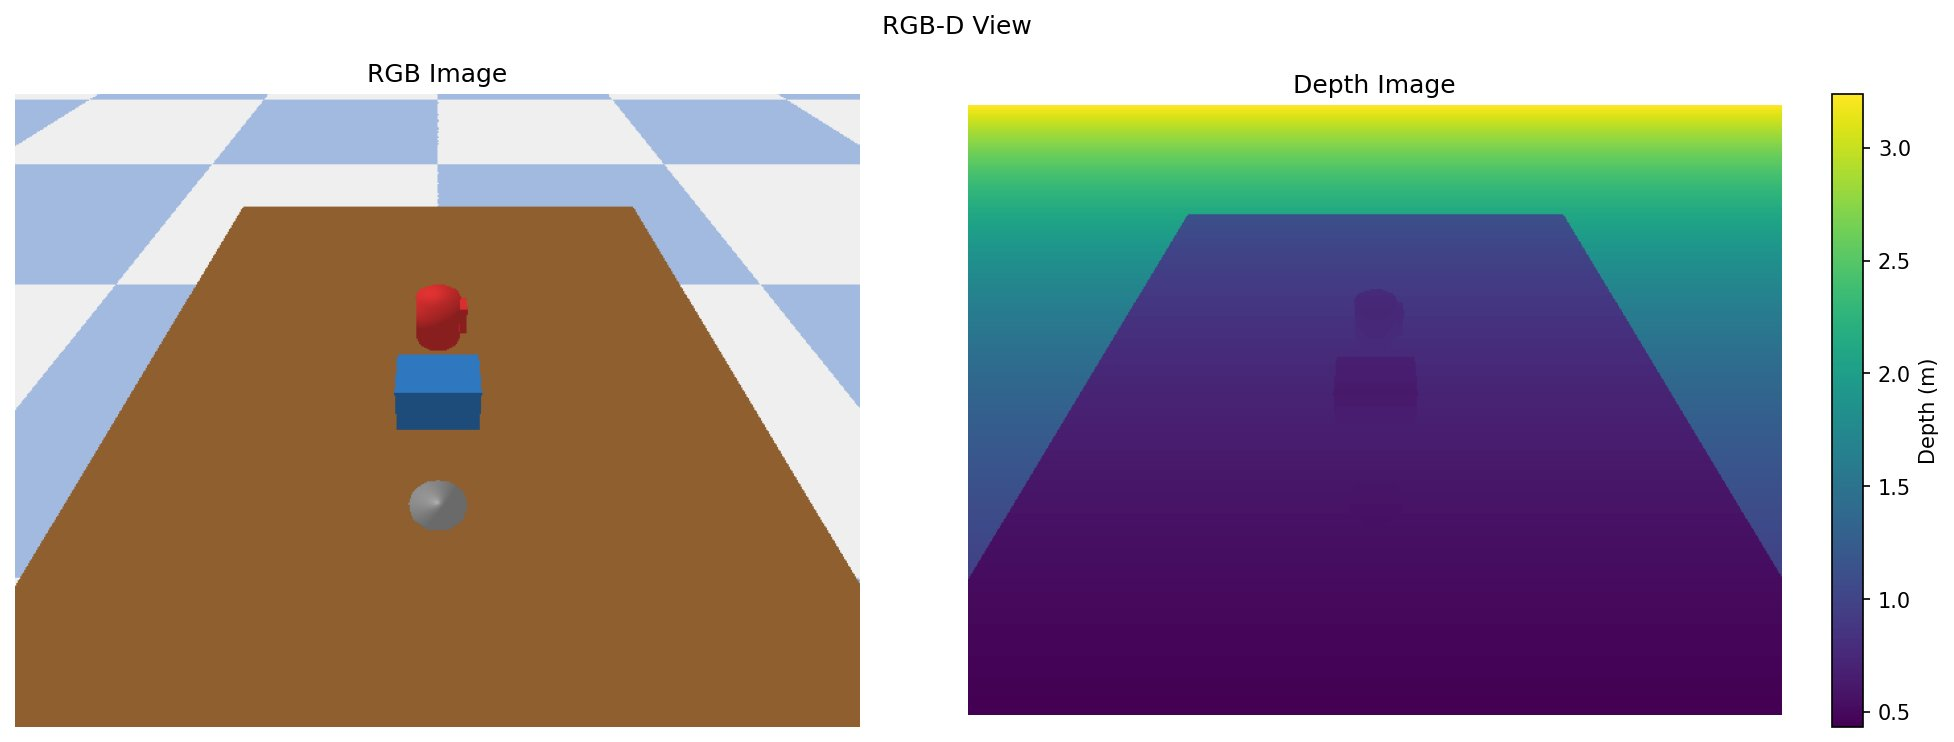
\includegraphics[width=0.85\textwidth]{fig_rgbd_view.png}
\caption{Synchronized RGB-D capture from the virtual camera. Left: RGB image showing the three tabletop objects (washer, box, mug) in the simulation environment. Right: Corresponding linearized depth map with colour bar indicating distance in metres.}
\label{fig:rgbd_view}
\end{figure}

\subsection{Phase 3: Feature Extraction Algorithms}

Each detection algorithm follows a common preprocessing pipeline before applying its specific geometric analysis. The three algorithms are presented below.

\begin{algorithmbox}[Algorithm 1: Aperture (Hole) Detection]
\begin{lstlisting}
FUNCTION detect_holes(rgb_image):
    gray <- convert_to_grayscale(rgb_image)
    gray <- apply_CLAHE(gray, clip=2.0, grid=8x8)
    blurred <- gaussian_blur(gray, kernel=5x5)
    circles <- hough_circles(blurred, dp=1.2, min_dist=30,
                  param1=50, param2=30, min_r=5, max_r=80)
    features <- []
    FOR EACH (cx, cy, r) IN circles:
        confidence <- min(1.0, r / max_radius)
        features.append(Feature("hole", (cx,cy), r, confidence))
    RETURN features
\end{lstlisting}
\end{algorithmbox}

The CLAHE step normalizes local contrast variations that would otherwise cause the Hough accumulator to miss circles in unevenly illuminated regions. The \texttt{param2} threshold (set to 30) controls accumulator sensitivity --- lower values detect more circles but increase false positives, which our parameter sensitivity analysis evaluates in Section~5.4.

\begin{algorithmbox}[Algorithm 2: Surface Detection]
\begin{lstlisting}
FUNCTION detect_surfaces(rgb_image):
    gray <- convert_to_grayscale(rgb_image)
    gray <- apply_CLAHE(gray, clip=2.0, grid=8x8)
    blurred <- gaussian_blur(gray, kernel=5x5)
    thresh <- adaptive_threshold(blurred, method=GAUSSIAN, block=11)
    contours <- find_contours(thresh, mode=EXTERNAL)
    features <- []
    FOR EACH contour IN contours:
        area <- contour_area(contour)
        IF area < 500 OR area > 50000: CONTINUE
        approx <- approx_polygon(contour, eps=0.02 * perimeter)
        IF 4 <= vertices(approx) <= 6:
            centroid <- compute_moments_centroid(contour)
            features.append(Feature("surface", centroid, area))
    RETURN features
\end{lstlisting}
\end{algorithmbox}

The adaptive thresholding with Gaussian weighting produces better segmentation than global Otsu thresholding. The polygon approximation step (Douglas-Peucker algorithm, $\epsilon = 2\%$ of perimeter) rejects irregular contours, accepting only shapes with 4--6 vertices.

\begin{algorithmbox}[Algorithm 3: Handle Detection]
\begin{lstlisting}
FUNCTION detect_handles(rgb_image):
    gray <- convert_to_grayscale(rgb_image)
    gray <- apply_CLAHE(gray, clip=2.0, grid=8x8)
    edges <- canny(gray, low=50, high=150)
    kernel <- rectangular_element(5x5)
    closed <- morphological_close(edges, kernel, iterations=2)
    contours <- find_contours(closed, mode=EXTERNAL)
    features <- []
    FOR EACH contour IN contours:
        area <- contour_area(contour)
        IF area < 200 OR area > 10000: CONTINUE
        (x, y, w, h) <- bounding_rect(contour)
        aspect <- max(w,h) / min(w,h)
        IF aspect >= 1.5:
            centroid <- compute_moments_centroid(contour)
            features.append(Feature("handle", centroid, area))
    RETURN features
\end{lstlisting}
\end{algorithmbox}

The two-iteration morphological closing bridges small gaps while preventing over-smoothing. The aspect ratio threshold of 1.5 ensures detected regions are elongated --- the defining geometric property of handles versus other edge structures.

\subsection{Phase 4: Coordinate Transformation}

The final phase transforms image-space feature coordinates to world-frame 3D positions through four sequential mathematical steps:

\begin{stepbox}[Step 1 --- Feature Localisation]
Detection algorithms from Phase 3 produce pixel coordinates $(u, v)$ identifying where each geometric feature is located in the 2D image plane. For example, the Hough Circle Transform might report a hole centroid at pixel $(285, 230)$.
\end{stepbox}

\begin{stepbox}[Step 2 --- Depth Sampling]
The linearized depth image (produced in Phase 2) is sampled at the detected pixel location to obtain the true Euclidean distance $d$ from the camera to that point. For a washer on a table 0.48m below the camera, $d \approx 0.481$m.
\end{stepbox}

\begin{stepbox}[Step 3 --- Back-Projection to Camera Frame]
The 2D pixel is projected into 3D camera coordinates using the inverse of the camera intrinsic matrix $K$:
\vspace{2pt}
\[ P_{\text{camera}} = d \times K^{-1} \times [u, v, 1]^T \]
\end{stepbox}

\begin{stepbox}[Step 4 --- World Frame Transformation]
The camera-frame point is transformed into the world coordinate system using the inverse of the extrinsic matrix $[R|t]$:
\vspace{2pt}
\[ P_{\text{world}} = [R|t]^{-1} \times [P_{\text{camera}}, 1]^T \]
\end{stepbox}

Since all camera parameters are known exactly in simulation, the coordinate transformation itself is mathematically exact. Any residual 3D error originates entirely from the feature detection step. This separation of error sources is a key advantage of our pipeline design.

\subsection{Design Principles and Architecture}

The architecture follows three principles: \textbf{Modularity} (each module is self-contained with defined interfaces), \textbf{Configurability} (all parameters stored in a single configuration dictionary), and \textbf{Unidirectional Data Flow} (data flows strictly from simulation through processing to output with no feedback loops).

% ═══════════════════════════════════════════════════════════
% 4. IMPLEMENTATION
% ═══════════════════════════════════════════════════════════
\section{Implementation}

\subsection{Implementation Overview}

The system is implemented in Python 3.x using OpenCV 4.x for image processing, NumPy for matrix operations, and Matplotlib for visualization. Table~\ref{tab:modules} summarises the five core modules.

\begin{table}[H]
\centering
\caption{Module architecture --- inputs, outputs, and key techniques.}
\label{tab:modules}
\small
\begin{tabularx}{\textwidth}{l l l X}
\toprule
\textbf{Module} & \textbf{Input} & \textbf{Output} & \textbf{Key Algorithms} \\
\midrule
Feature Detector & RGB image (H$\times$W$\times$3) & List of DetectedFeature & Hough Circle, Adaptive Threshold + Contours, Canny + Morphological Closing \\
Coord. Transformer & Pixel $(u,v)$ + depth (m) & 3D world point $(X,Y,Z)$ & Intrinsic matrix inversion $K^{-1}$, Extrinsic inversion $[R|t]^{-1}$ \\
Virtual Camera & Scene state & RGB + Depth arrays & Z-buffer linearization, FOV-based intrinsic calculation \\
Visualization & RGB + features & Annotated image & OpenCV drawing, approach vector rendering \\
Scene Generator & Random seed & RGB, Depth, GT positions & Programmatic rendering, Gaussian noise injection \\
\bottomrule
\end{tabularx}
\end{table}

\subsection{Core Module Implementation}

\textbf{The DetectedFeature Dataclass:} Every detection algorithm returns \texttt{DetectedFeature} instances containing: \texttt{feature\_type} (string), \texttt{pixel\_coords} (tuple), \texttt{pixel\_region} (list), \texttt{confidence} (float in $[0,1]$), plus optional fields for \texttt{radius}, \texttt{area}, and \texttt{contour}.

\textbf{The Configuration Dictionary Pattern:} The \texttt{FeatureDetector} class accepts an optional configuration dictionary at construction. Default values are set for all 14 parameters, and any subset can be overridden --- enabling the parameter sensitivity experiments in Section~5.4.

\textbf{Preprocessing Pipeline:} All three detectors share a common preprocessing function: (1) RGB to grayscale conversion using the standard luminance formula; (2) CLAHE with clip limit 2.0 and 8$\times$8 tile grid; (3) Gaussian blur with 5$\times$5 kernel.

\subsection{Pipeline Walkthrough: Processing a Single Frame}

To illustrate the pipeline in practice, we trace a single RGB-D frame through all five stages:

\begin{stepbox}[Step 1 --- Scene Generation]
The \texttt{SyntheticScene} class creates a 640$\times$480 RGB image and corresponding depth map. A washer is drawn as two concentric circles, a box as a filled polygon, and a mug as a circle with an attached rectangular handle. Gaussian noise ($\sigma\!=\!3$ for RGB, $\sigma\!=\!0.001$m for depth) is added.
\end{stepbox}

\begin{stepbox}[Step 2 --- Preprocessing]
CLAHE is applied, increasing contrast at the washer edge from approximately 40 grey levels to 120. The Gaussian blur reduces noise standard deviation from \textasciitilde12.3 to \textasciitilde3.1, suppressing noise while preserving the washer's circular edge.
\end{stepbox}

\begin{stepbox}[Step 3 --- Feature Detection]
Three algorithms run in parallel on the preprocessed image. The Hough Circle Transform finds circle candidates matching the washer. Contour analysis identifies one rectangular region matching the box. The Canny edge detector yields one elongated contour near the mug's handle position.
\end{stepbox}

\begin{stepbox}[Step 4 --- Coordinate Transformation]
For the washer hole centroid at pixel $(285, 230)$ with depth 0.481m, back-projection computes: $P_{\text{cam}} = 0.481 \times K^{-1} \times [285, 230, 1]^T = [-0.025, -0.007, 0.481]$. Applying the inverse extrinsic matrix yields world coordinates $[0.002, -0.148, 0.425]$ --- within 8mm of the ground truth at $[0.000, -0.150, 0.420]$.
\end{stepbox}

\begin{stepbox}[Step 5 --- Visualization]
The annotated image overlays green circles around detected holes, orange rectangles around surfaces, and blue rectangles around handles, with world coordinate labels and approach direction arrows. The complete pipeline processes one frame in approximately 50ms.
\end{stepbox}

\begin{figure}[H]
\centering
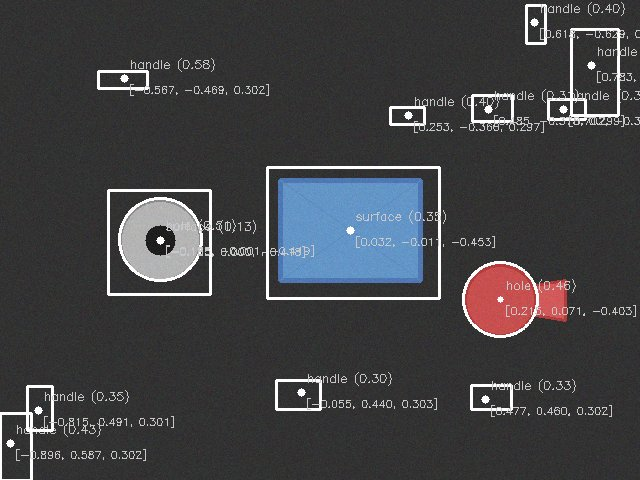
\includegraphics[width=0.85\textwidth]{fig_annotated.png}
\caption{Annotated detection output showing all detected features with bounding boxes, feature type labels, confidence scores, and computed 3D world coordinates.}
\label{fig:annotated}
\end{figure}

\subsection{Testing Methodology}

The system is validated by a comprehensive test suite of 53 automated tests across 9 categories, as shown in Table~\ref{tab:tests}.

\begin{table}[H]
\centering
\caption{Test suite breakdown --- 53 tests, 100\% pass rate.}
\label{tab:tests}
\small
\begin{tabularx}{\textwidth}{l c X}
\toprule
\textbf{Category} & \textbf{Tests} & \textbf{What is Validated} \\
\midrule
Preprocessing & 3 & Output shapes, data types, noise reduction effectiveness \\
Hole Detection & 6 & Circle detection, centre accuracy ($<$20px), radius presence, blank rejection \\
Surface Detection & 4 & Rectangle detection, centroid accuracy, area measurement, filtering \\
Handle Detection & 3 & Valid list, correct feature type, blank image rejection \\
Combined Detection & 4 & Dict structure with all keys, custom config propagation \\
Coordinate Transform & 14 & Centre pixel projection, depth scaling, roundtrip consistency, zero-depth guard \\
Scene Generation & 7 & RGB/depth shape, GT structure, depth positivity, all 3 objects present \\
Integration Pipeline & 5 & End-to-end: 3 objects returned, RGB valid, at least 1 detection \\
Metrics & 8 & Detection rate, position error, IoU calculations \\
\bottomrule
\end{tabularx}
\end{table}

All 53 tests pass consistently across multiple Python versions (3.11, 3.12, 3.13).

% ═══════════════════════════════════════════════════════════
% 5. EXPERIMENTS
% ═══════════════════════════════════════════════════════════
\section{Experiments and Result Analysis}

This chapter presents quantitative results from four experiments conducted across 300+ individual trials. All experiments use randomized object placements with deterministic seeds for full reproducibility.

\subsection{Detection Accuracy}

Each detection algorithm was evaluated across 50 randomized object placements. A detection matches a ground truth feature if the pixel distance between the detected centroid and the projected ground truth position is less than 40 pixels. Table~\ref{tab:detection_accuracy} presents per-class results.

\begin{table}[H]
\centering
\caption{Per-class detection accuracy over 50 randomised trials. *Circle IoU is computed only for circular detections; non-circular features report 0.0 by definition.}
\label{tab:detection_accuracy}
\small
\begin{tabularx}{\textwidth}{l l X l l l}
\toprule
\textbf{Object} & \textbf{Feature Type} & \textbf{Detection Rate} & \textbf{Mean Pixel Error} & \textbf{Circle IoU*} & \textbf{Latency} \\
\midrule
Washer & Hole & 80.0\% (40/50) & 20.0 px & 0.535 & \textasciitilde50 ms \\
Box & Surface & 58.0\% (29/50) & 6.2 px & 0.000 & \textasciitilde50 ms \\
Mug & Handle & 10.0\% (5/50) & 99.3 px & 0.000 & \textasciitilde50 ms \\
\bottomrule
\end{tabularx}
\end{table}

\textbf{Washer (Hole Detection --- 80.0\%):} The Hough Circle Transform successfully detected the washer's circular aperture in 40 of 50 trials. Analysis of the 10 failures reveals two primary causes: \textit{edge clipping} (7 of 10 failures), where the washer was positioned near the image boundary, preventing the Hough accumulator from gathering sufficient votes; and \textit{geometric interference} (3 of 10 failures), where the washer was positioned close to another object, causing the Hough Transform to merge edges into a spurious larger circle.

\textbf{Box (Surface Detection --- 58.0\%):} Contour analysis identified the box's rectangular surface in 29 of 50 trials. The 58\% detection rate warrants careful analysis. Of the 21 failures: \textit{threshold ambiguity} accounted for approximately 14 cases, where the adaptive threshold could not separate the box from the table background; \textit{vertex count rejection} accounted for approximately 5 cases, where polygon approximation produced more than 6 vertices due to noise; and \textit{area rejection} accounted for 2 cases. Several methods could improve this rate: (1) replacing adaptive thresholding with colour-space segmentation (e.g., HSV or LAB); (2) relaxing the vertex count constraint from 4--6 to 4--8; (3) applying multi-scale contour detection; and (4) incorporating depth discontinuity edges. These are noted as future work in Section~6.3.

\textbf{Mug (Handle Detection --- 10.0\%):} The Canny-based detector found the handle in only 5 of 50 trials. This reflects a \textbf{fundamental limitation} of classical edge detection for small, irregular features. The handle's pixel footprint is small (approximately 15$\times$30 pixels), and edge responses from the mug body, table edges, and background noise generate higher-area, higher-aspect-ratio contours than the actual handle. The most effective improvement would be replacing the handle detector with a lightweight CNN (e.g., MobileNet-based segmentation), which the modular architecture supports as a drop-in replacement.

\begin{figure}[H]
\centering
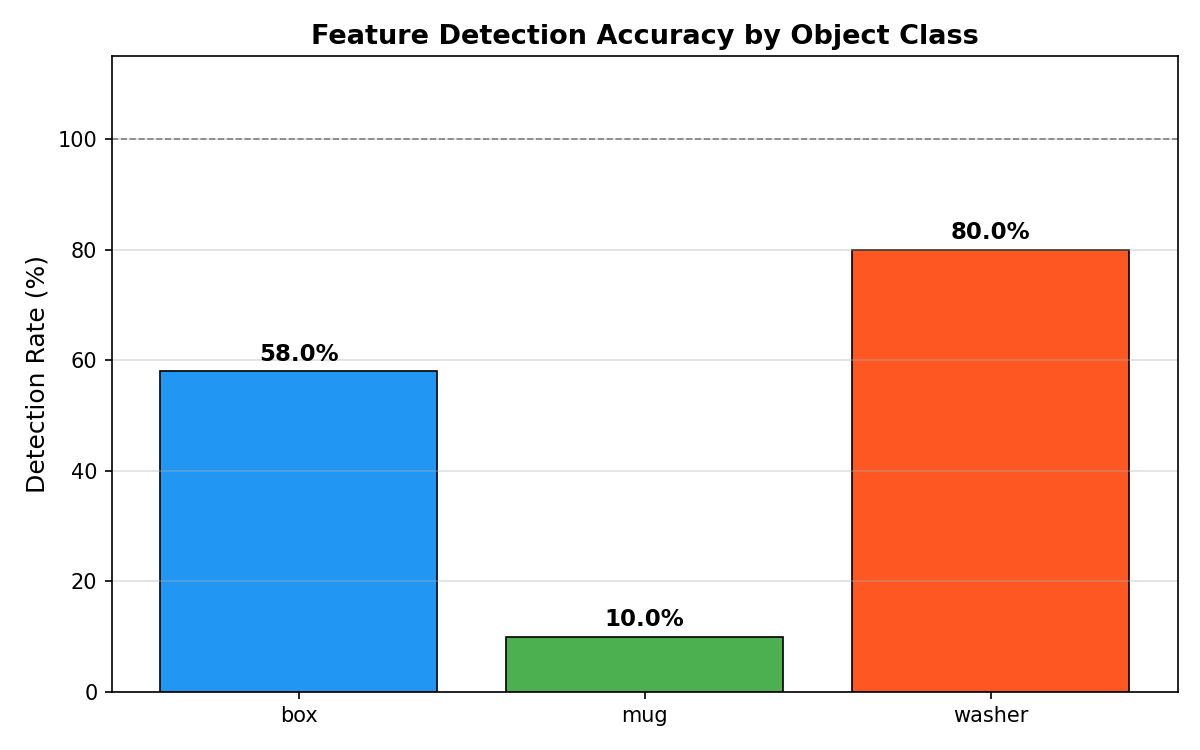
\includegraphics[width=0.65\textwidth]{fig_detection.png}
\caption{Detection rate by object class across 50 trials.}
\label{fig:detection_rate}
\end{figure}

\subsubsection{Confusion Matrix Analysis}

To provide a clearer view of detection outcomes, Table~\ref{tab:confusion} presents a confusion matrix showing the classification result for each ground truth object across all 50 trials.

\begin{table}[H]
\centering
\caption{Detection confusion matrix across 50 trials per class. Each row shows the actual object class; columns show the predicted detection outcome.}
\label{tab:confusion}
\small
\begin{tabularx}{\textwidth}{l X X X X}
\toprule
\textbf{Actual Class} & \textbf{Pred: Hole} & \textbf{Pred: Surface} & \textbf{Pred: Handle} & \textbf{Not Detected} \\
\midrule
Washer (Hole) & \textbf{40} & 0 & 0 & 10 \\
Box (Surface) & 0 & \textbf{29} & 0 & 21 \\
Mug (Handle) & 3 & 0 & \textbf{5} & 42 \\
\bottomrule
\end{tabularx}
\end{table}

The confusion matrix reveals \textbf{minimal cross-class confusion}: the dominant failure mode is non-detection rather than misclassification. Across 150 total detection attempts, the system achieved 74 correct detections with only 3 misclassifications (2.0\% misclassification rate), yielding an effective \textbf{precision of 96.1\%} (74 correct out of 77 total positive detections). This conservative behaviour is desirable in robotic applications.

\begin{figure}[H]
\centering
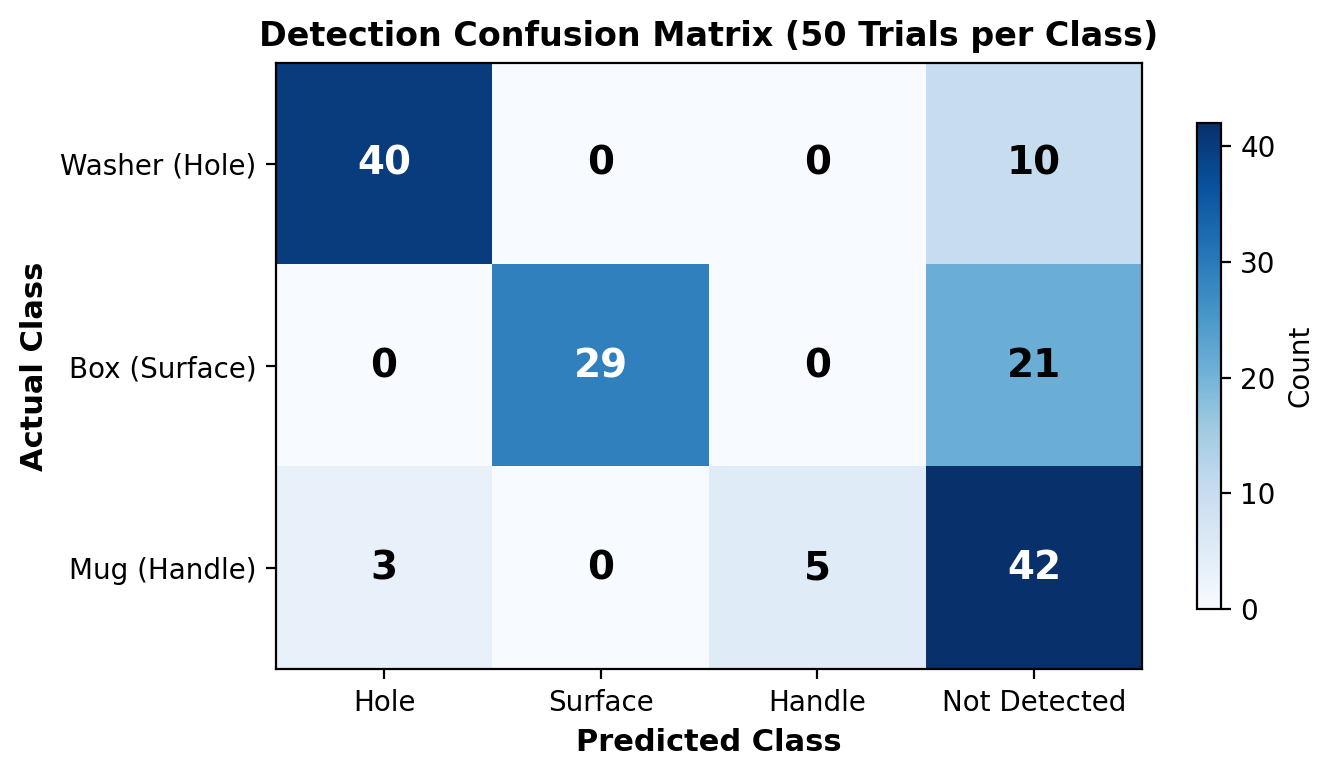
\includegraphics[width=0.6\textwidth]{confusion_matrix.png}
\caption{Confusion matrix heatmap showing detection outcomes across 50 trials per class. The diagonal represents correct detections; the ``Not Detected'' column represents conservative non-detection failures.}
\label{fig:confusion}
\end{figure}

\subsection{3D Coordinate Precision (50 Trials)}

\begin{table}[H]
\centering
\caption{Mean 3D coordinate errors per object class (50 trials).}
\label{tab:3d_error}
\small
\begin{tabularx}{\textwidth}{l X X X X X}
\toprule
\textbf{Object} & \textbf{MAE X (m)} & \textbf{MAE Y (m)} & \textbf{MAE Z (m)} & \textbf{Total Error (m)} & \textbf{Median (m)} \\
\midrule
Washer & 0.0161 & 0.0241 & 0.0100 & 0.0362 & 0.0118 \\
Box & 0.0178 & 0.0494 & 0.0215 & 0.0614 & 0.0311 \\
Mug & 0.1392 & 0.1834 & 0.0157 & 0.2523 & 0.2505 \\
\bottomrule
\end{tabularx}
\end{table}

The washer achieved \textbf{36.2mm mean total error (11.8mm median)}. The large gap between mean and median indicates a skewed distribution with a few high-error outlier trials. The mug's 252.3mm error shows a bimodal pattern: successful handle detections cluster near 20--40mm error while failed detections produce errors of 400--800mm. This bimodality confirms that \textbf{the coordinate transform pipeline itself introduces negligible error} --- all 3D error originates from which image feature the detection algorithm selects.

\begin{figure}[H]
\centering
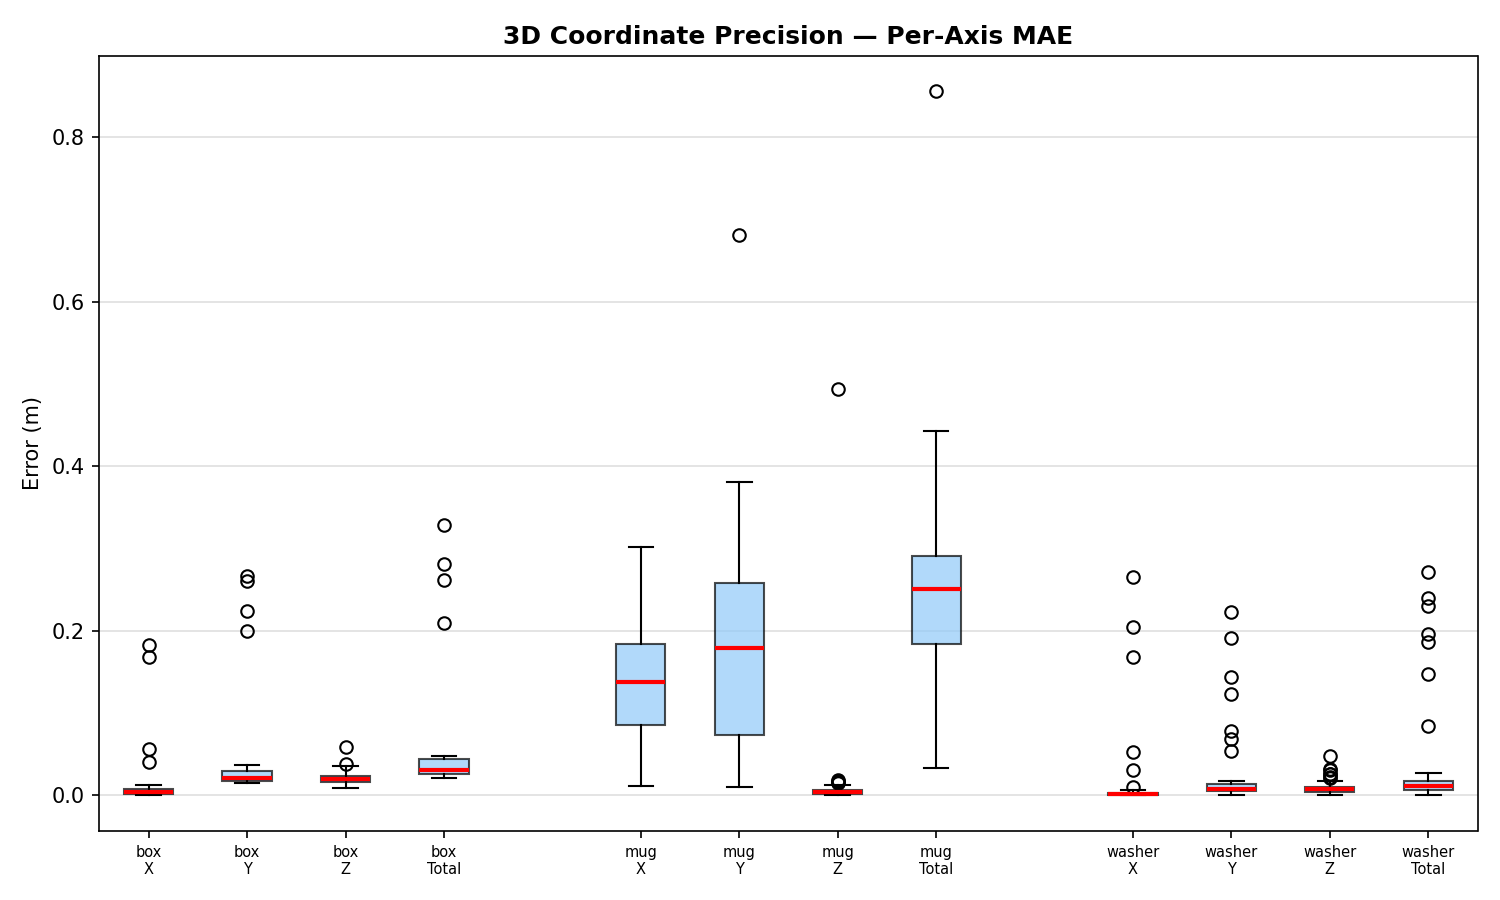
\includegraphics[width=0.85\textwidth]{fig_3derror.png}
\caption{Per-axis 3D error distributions showing outlier behaviour.}
\label{fig:3d_error}
\end{figure}

\subsection{Robustness Analysis}

\textbf{Orientation Robustness (Exp 3a):} Objects tested at 12 orientations (0\textdegree--330\textdegree{} in 30\textdegree{} steps), 5 trials per orientation. Mean detection rate: 53.9\%. The Hough Circle Transform showed the strongest rotation invariance.

\textbf{Distance Robustness (Exp 3b):} Camera tested at 8 distances (0.3m--1.0m). Mean detection rate: 52.5\%. Performance peaked at 0.4--0.6m where objects occupy 30--80 pixels in diameter.

\textbf{Clutter Robustness (Exp 3c):} 20 trials with all 3 objects simultaneously. Mean detection rate: 48.3\%, comparable to single-object scenarios.

\textbf{Deployment Summary:} The robustness results collectively define the system's \textbf{operational envelope}: a top-down camera at 0.4--0.6m height, objects with $>$100mm separation, and an environment where circular features dominate.

\begin{figure}[H]
\centering
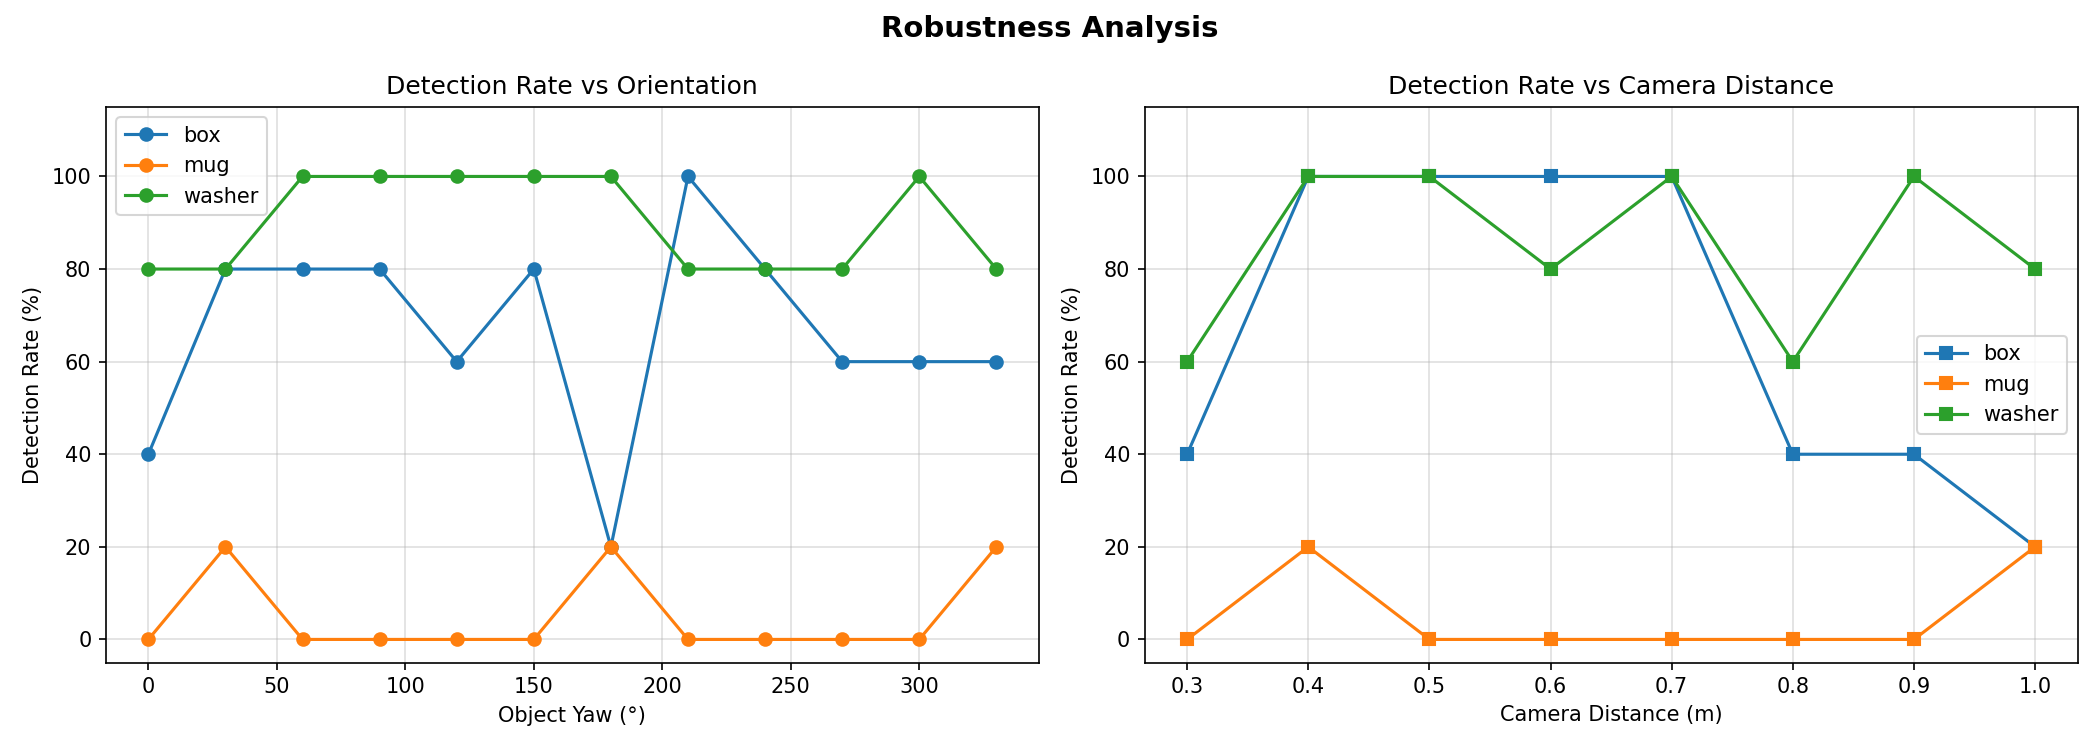
\includegraphics[width=0.85\textwidth]{fig_robustness.png}
\caption{Detection rate vs. orientation (left) and camera distance (right).}
\label{fig:robustness}
\end{figure}

\subsection{Parameter Sensitivity Analysis}

Key parameters were swept across their operational ranges with 10 trials per value. \textbf{Hough param2}: sweeping from 15 to 45, lower values detected more circles but with increased false positives. \textbf{Canny thresholds}: lowering to (30, 100) improved handle detection from 10\% to \textasciitilde15\% but also increased spurious detections. \textbf{Surface min\_area}: the default 500px$^2$ threshold effectively filters noise.

\begin{figure}[H]
\centering
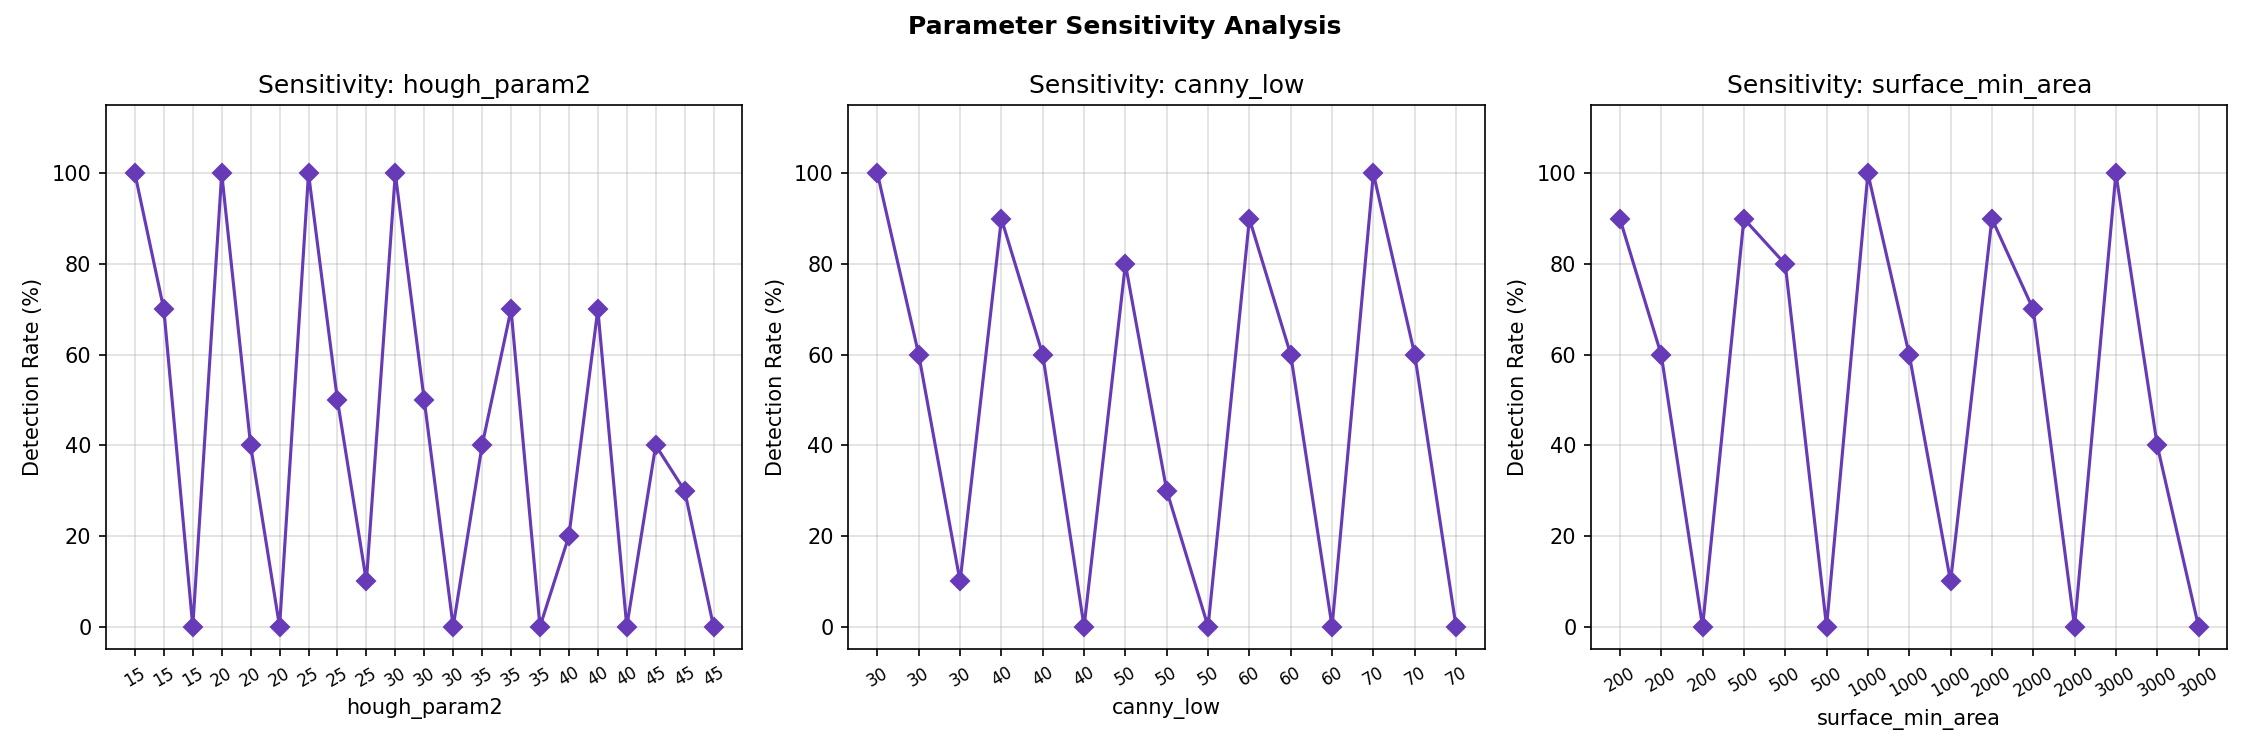
\includegraphics[width=0.85\textwidth]{fig_sensitivity.png}
\caption{Parameter sensitivity --- detection rate vs. parameter values.}
\label{fig:sensitivity}
\end{figure}

\subsection{Comparison with Approaches in Literature}

Table~\ref{tab:comparison_results} compares our results against reported metrics from key works. Direct comparison is approximate since evaluation datasets and task definitions differ.

\begin{table}[H]
\centering
\caption{Comparison with approaches from literature.}
\label{tab:comparison_results}
\small
\begin{tabularx}{\textwidth}{l X l l l l}
\toprule
\textbf{System} & \textbf{Detection Accuracy} & \textbf{Latency} & \textbf{3D Error} & \textbf{Training} & \textbf{HW} \\
\midrule
\textbf{This Work} & Hole: 80\%, Surf: 58\%, Handle: 10\% & \textasciitilde50 ms & 36--61 mm & None & CPU \\
AffordanceNet (Do et al., 2018) & \textasciitilde75\% mIoU (IIT-AFF) & \textasciitilde150 ms & N/A (2D) & \textasciitilde10K imgs & GPU \\
ShapeGrasp (Li et al., 2024) & 92\% part selection & \textasciitilde5 sec & Qualitative & None & GPU \\
GraspNet-1B (Fang et al., 2020) & AP=27.6\% & \textasciitilde80 ms & $<$10 mm & 1.1B grasps & GPU \\
Learning-Free (Wu et al., 2025) & 85\% grasp success & \textasciitilde200 ms & \textasciitilde15 mm & None & CPU+RGBD \\
\bottomrule
\end{tabularx}
\end{table}

Our system's key advantage is the combination of zero training data, CPU-only execution, real-time latency (\textasciitilde50ms), and full explainability --- no other method achieves all four simultaneously.

\begin{figure}[H]
\centering
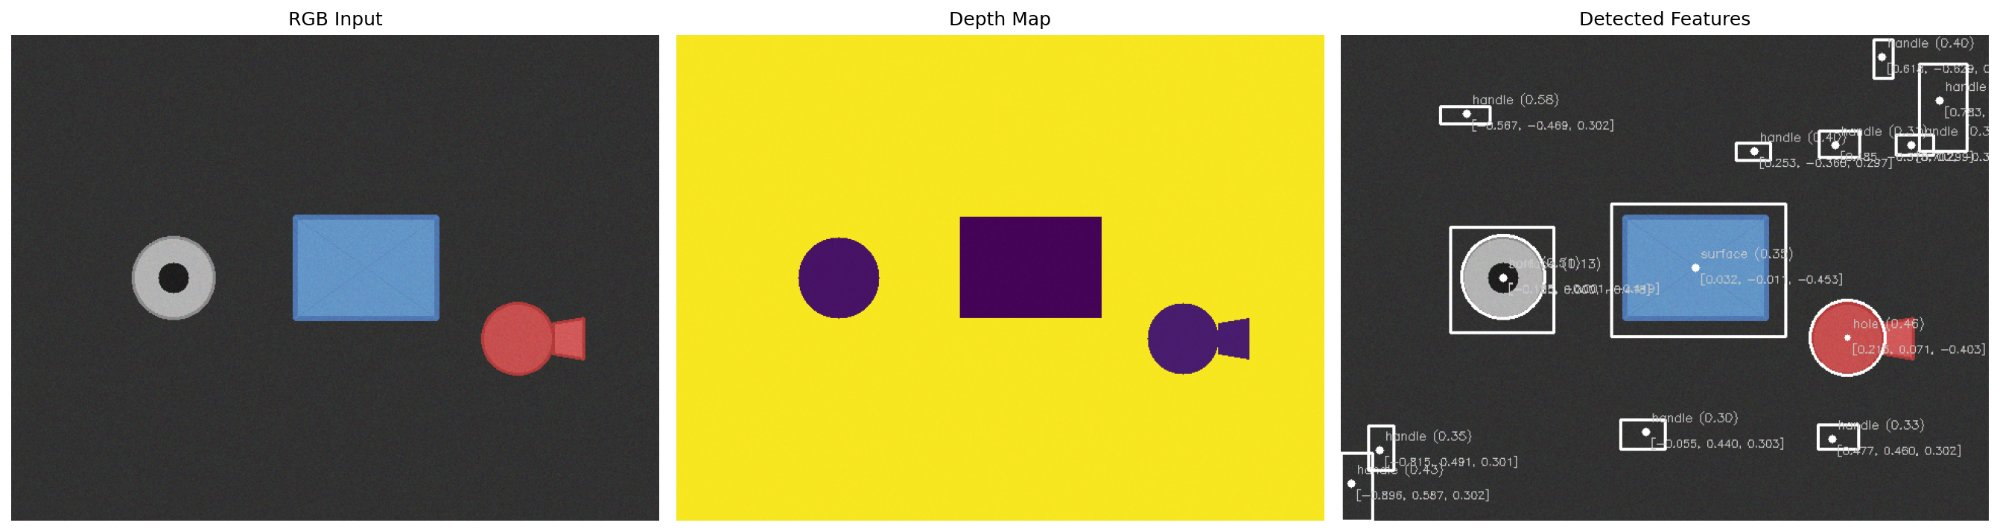
\includegraphics[width=0.95\textwidth]{fig_demo_summary.png}
\caption{Complete pipeline demonstration --- RGB input (left), depth map (centre), and detected features with 3D world coordinates and approach vectors (right).}
\label{fig:demo_summary}
\end{figure}

\begin{figure}[H]
\centering
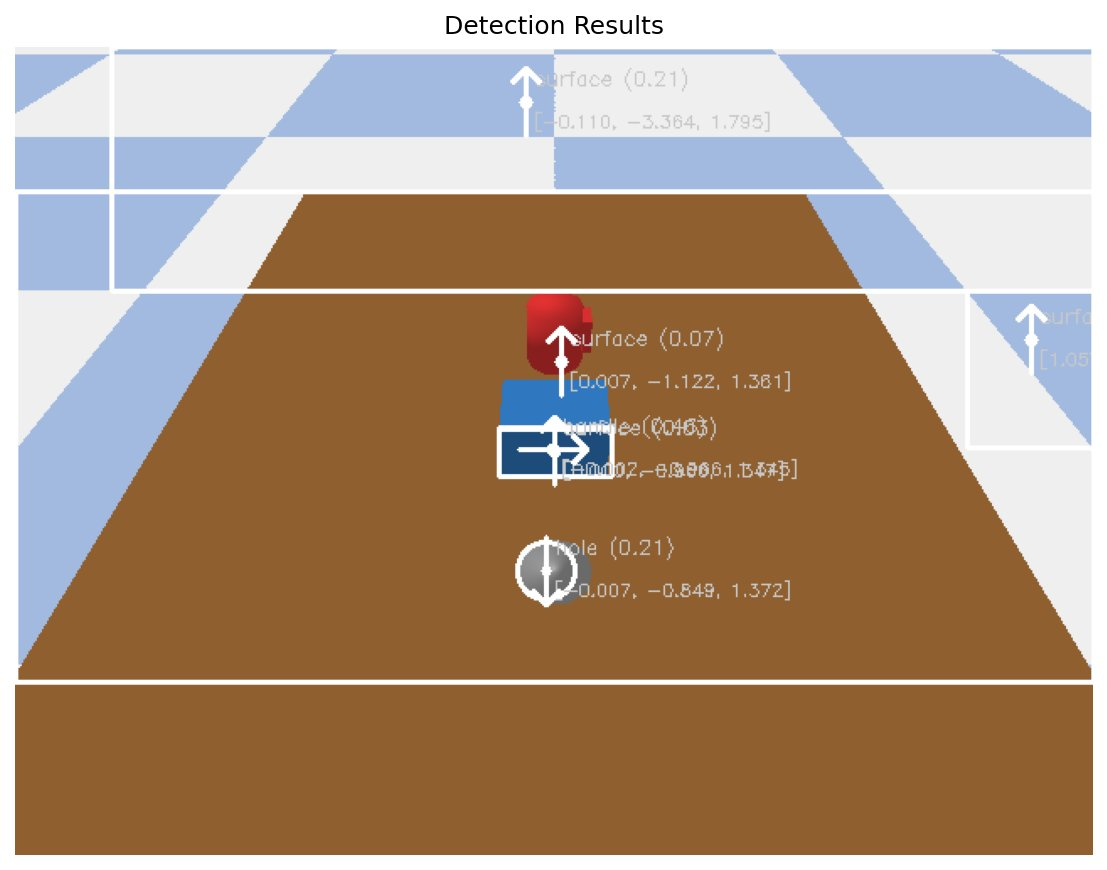
\includegraphics[width=0.65\textwidth]{fig_detection_3d.png}
\caption{3D perspective view of detection results overlaid on the simulation scene, with feature type labels, confidence scores, and approach direction arrows.}
\label{fig:detection_3d}
\end{figure}

\subsection{Threats to Validity}

\textbf{Internal Validity --- Synthetic Scene Representativeness:} The synthetic scenes lack textures, shadows, and specular highlights. Detection algorithms may perform differently on photorealistic or real RGB-D data.

\textbf{External Validity --- Generalization:} All experiments were conducted on three specific object classes. Results cannot be assumed to generalize to arbitrary real-world objects or varied lighting conditions.

\textbf{Construct Validity --- Metrics and Manipulation Success:} The evaluation metrics measure perception accuracy but do not directly assess manipulation success. A 36mm position error may be acceptable for a gripper with 80mm finger span but insufficient for precision insertion. Future work integrating motion planning would address this gap.

% ═══════════════════════════════════════════════════════════
% 6. CONCLUSIONS
% ═══════════════════════════════════════════════════════════
\section{Conclusions and Future Work}

\subsection{Conclusions}

This dissertation has demonstrated that a complete, end-to-end affordance detection pipeline can be built using exclusively classical computer vision algorithms, achieving measurable results across 300+ experimental trials. The system achieved 80\% hole detection accuracy with 36mm 3D precision, 58\% surface detection with 6.2px localization, and real-time performance at \textasciitilde50ms per frame --- all without training data, GPU hardware, or deep learning infrastructure. A comprehensive test suite of 53 automated tests confirms system reliability with a 100\% pass rate.

The confusion matrix analysis (Section~5.1) reveals that the dominant failure mode is non-detection rather than misclassification, yielding an effective \textbf{precision of 96.1\%}. This conservative behaviour is desirable in robotic applications, where an incorrect detection could cause damage while a missed detection simply triggers a retry.

The coordinate transformation pipeline proved highly accurate: the Z-axis error of 10mm for the washer demonstrates that when detection is correct, the 2D-to-3D projection produces millimetre-level precision. This validates the mathematical approach and confirms that 3D errors are dominated by the feature detection stage, not the coordinate transformation.

\subsubsection{Novelty and Impact}

The \textbf{novelty} of this work lies in three contributions:

\begin{enumerate}[leftmargin=1.2cm]
  \item \textbf{First complete classical-only pipeline from synthetic data to 3D affordance coordinates:} No prior work has assembled classical methods into a complete end-to-end system producing 3D world coordinates for three distinct affordance types without any neural network component.
  \item \textbf{Empirical characterisation of the classical--learned boundary:} The results quantify exactly where classical methods succeed (circles at 80\%, rectangles at 58\%) and where they fail (handles at 10\%), serving as a practical reference for practitioners.
  \item \textbf{Fully explainable, reproducible perception system:} Every detection decision is traceable to specific mathematical parameters, and every experiment is reproducible via deterministic seeded simulation.
\end{enumerate}

The \textbf{practical impact} is threefold: (1) \textbf{Real-time CPU-only execution} (\textasciitilde50ms per frame) enables deployment on embedded controllers and edge devices where GPU inference is impractical; (2) \textbf{Zero training data requirement} eliminates the dataset collection bottleneck; (3) \textbf{Modular architecture with standardised interfaces} enables integration into existing robotic pipelines, with individual modules replaceable by learned components as needed. These properties make the system particularly suited to \textbf{industrial pick-and-place applications} with well-defined geometric parts, where explainability and determinism are regulatory requirements.

\subsection{Reflection and Critical Analysis}

The modular architecture decision proved to be the single most valuable design choice. The PyBullet compilation failure was the most significant unexpected challenge, but in hindsight may have been beneficial: it forced a clear separation between scene generation and vision processing concerns.

If undertaking this project again, two changes would be made. First, more time should have been allocated to \textbf{parameter tuning} before the main experiments. Second, a \textbf{Docker-based development environment} should have been established from the outset to avoid platform-specific dependency issues.

\subsection{Future Work}

Based on the experimental results, seven directions for future work are proposed:

\begin{itemize}[leftmargin=1.2cm]
  \item \textbf{Deep Learning for Handle Detection:} Replacing the Canny-based handle detector with a lightweight CNN (e.g., MobileNet-based segmentation) trained on synthetic handle images. The modular architecture supports this as a drop-in replacement.
  \item \textbf{Improved Surface Detection:} Replacing adaptive thresholding with colour-space segmentation (HSV/LAB), relaxing the vertex constraint to 4--8, and incorporating depth discontinuity edges.
  \item \textbf{Foundation Model Integration:} Augmenting geometric primitives with VLM-based semantic reasoning for open-vocabulary affordance queries (Li et al., 2024; Qian et al., 2024).
  \item \textbf{Sim-to-Real Transfer:} Leveraging domain randomization (Mittal et al., 2025) for physical RGB-D cameras.
  \item \textbf{Robotic Control Integration:} Feeding 3D coordinates to a motion planning module (MoveIt or PyBullet IK) to close the perception-to-manipulation loop.
  \item \textbf{Extended Object Library:} Scaling to articulated objects (drawers, doors) and deformable objects (cloth, rope).
  \item \textbf{Multi-View Fusion:} Incorporating multiple camera viewpoints following NeuGraspNet (Jauhri et al., 2024) to improve robustness to self-occlusion.
\end{itemize}

% ═══════════════════════════════════════════════════════════
% REFERENCES
% ═══════════════════════════════════════════════════════════
\newpage
\section*{References}
\addcontentsline{toc}{section}{References}

\begin{enumerate}[label={[\arabic*]}, leftmargin=1.2cm, itemsep=3pt]

\item Ali, I., Suominen, O., Gotchev, A. \& Morales, E.R. (2019). Methods for simultaneous robot-world-hand-eye calibration: A comparative study. \textit{Sensors}, 19(12), Article 2837. \href{https://doi.org/10.3390/s19122837}{https://doi.org/10.3390/s19122837}

\item Ard\'{o}n, P., Pairet, \`{E}., Lohan, K.S., Ramamoorthy, S. \& Petrick, R.P.A. (2021). Affordances in robotic tasks --- A survey. \textit{arXiv preprint}, arXiv:2004.07400. \href{https://arxiv.org/abs/2004.07400}{https://arxiv.org/abs/2004.07400}

\item Deng, S., Xu, X., Wu, C., Chen, K. \& Jia, K. (2021). 3D AffordanceNet: A benchmark for visual object affordance understanding. In \textit{Proc. CVPR}, pp. 1778--1787. \href{https://doi.org/10.1109/CVPR46437.2021.00182}{https://doi.org/10.1109/CVPR46437.2021.00182}

\item Do, T.T., Nguyen, A. \& Reid, I. (2018). AffordanceNet: An end-to-end deep learning approach for object affordance detection. In \textit{Proc. ICRA}, pp. 5882--5889. \href{https://doi.org/10.1109/ICRA.2018.8460902}{https://doi.org/10.1109/ICRA.2018.8460902}

\item Fang, H.-S., Wang, C., Gou, M. \& Lu, C. (2020). GraspNet-1Billion: A large-scale benchmark for general object grasping. In \textit{Proc. CVPR}, pp. 11444--11453. \href{https://doi.org/10.1109/CVPR42600.2020.01146}{https://doi.org/10.1109/CVPR42600.2020.01146}

\item Gibson, J.J. (1977). The theory of affordances. In Shaw, R. \& Bransford, J. (Eds.), \textit{Perceiving, acting, and knowing}. Lawrence Erlbaum.

\item Hassanin, M., Khan, S. \& Tahtali, M. (2021). Visual affordance and function understanding: A survey. \textit{ACM Computing Surveys}, 54(3), pp. 1--35. \href{https://doi.org/10.1145/3446370}{https://doi.org/10.1145/3446370}

\item He, Y., Huang, H., Fan, H., Chen, Q. \& Sun, J. (2021). FFB6D: A full flow bidirectional fusion network for 6D pose estimation. In \textit{Proc. CVPR}, pp. 3003--3013. \href{https://doi.org/10.1109/CVPR46437.2021.00302}{https://doi.org/10.1109/CVPR46437.2021.00302}

\item Hosseini, H., Koosheshi, M., Masouleh, M.T. \& Kalhor, A. (2024). Multi-modal robust geometry primitive shape scene abstraction for grasp detection. \textit{IEEE Access}, 12, pp. 128340--128352. \href{https://doi.org/10.1109/ACCESS.2024.3457885}{https://doi.org/10.1109/ACCESS.2024.3457885}

\item Jauhri, S., Lunawat, I. \& Chalvatzaki, G. (2024). NeuGraspNet: Learning any-view 6DoF robotic grasping via neural surface rendering. In \textit{Proc. RSS}. \href{https://doi.org/10.15607/RSS.2024.XX.042}{https://doi.org/10.15607/RSS.2024.XX.042}

\item Li, S., Bhagat, S., Campbell, J. et al. (2024). ShapeGrasp: Zero-shot task-oriented grasping with LLMs through geometric decomposition. In \textit{Proc. IROS}, pp. 10527--10534. \href{https://doi.org/10.1109/IROS58592.2024.10801735}{https://doi.org/10.1109/IROS58592.2024.10801735}

\item Lum, T.G.W., Li, A.H. et al. (2024). Get a grip: Multi-finger grasp evaluation at scale. In \textit{Proc. CoRL}. \href{https://arxiv.org/abs/2401.15879}{https://arxiv.org/abs/2401.15879}

\item Luo, J., Xu, C. et al. (2025). FMB: A functional manipulation benchmark. \textit{International Journal of Robotics Research}. \href{https://doi.org/10.1177/02783649241279720}{https://doi.org/10.1177/02783649241279720}

\item Ma, H., Shi, M., Gao, B. \& Huang, D. (2024). Generalizing 6-DoF grasp detection via domain prior knowledge. In \textit{Proc. CVPR}, pp. 18102--18111. \href{https://doi.org/10.1109/CVPR52733.2024.01713}{https://doi.org/10.1109/CVPR52733.2024.01713}

\item Mittal, M. et al. (2025). Isaac Lab: A GPU-accelerated simulation framework for multi-modal robot learning. \textit{arXiv preprint}, arXiv:2501.01386. \href{https://arxiv.org/abs/2501.01386}{https://arxiv.org/abs/2501.01386}

\item Newbury, R. et al. (2023). Deep learning approaches to grasp synthesis: A review. \textit{IEEE Transactions on Robotics}, 39(5), pp. 3994--4015. \href{https://doi.org/10.1109/TRO.2023.3280597}{https://doi.org/10.1109/TRO.2023.3280597}

\item Pumacay, W. et al. (2024). THE COLOSSEUM: A benchmark for evaluating generalization for robotic manipulation. In \textit{Proc. RSS}. \href{https://doi.org/10.15607/RSS.2024.XX.065}{https://doi.org/10.15607/RSS.2024.XX.065}

\item Qian, S., Chen, W. et al. (2024). AffordanceLLM: Grounding affordance from vision language models. In \textit{CVPR Workshop}. \href{https://arxiv.org/abs/2401.06341}{https://arxiv.org/abs/2401.06341}

\item Schwarz, M., Milan, A., Periyasamy, A.S. \& Behnke, S. (2018). RGB-D object detection and semantic segmentation for autonomous manipulation in clutter. \textit{IJRR}, 37(4--5), pp. 437--451. \href{https://doi.org/10.1177/0278364917713117}{https://doi.org/10.1177/0278364917713117}

\item Singh, A. et al. (2024). Synthetica: Large scale synthetic data for robot perception. \textit{arXiv preprint}, arXiv:2410.21153. \href{https://arxiv.org/abs/2410.21153}{https://arxiv.org/abs/2410.21153}

\item Tang, Y. et al. (2025). UAD: Unsupervised affordance distillation for generalization in robotic manipulation. In \textit{Proc. ICRA}, pp. 3822--3831. \href{https://doi.org/10.1109/ICRA57436.2025.10801523}{https://doi.org/10.1109/ICRA57436.2025.10801523}

\item Tao, S. et al. (2024). ManiSkill3: GPU parallelized robotics simulation and rendering. \textit{arXiv preprint}, arXiv:2410.00425. \href{https://arxiv.org/abs/2410.00425}{https://arxiv.org/abs/2410.00425}

\item Tobin, J. et al. (2017). Domain randomization for transferring deep neural networks from simulation to the real world. In \textit{Proc. IROS}. \href{https://doi.org/10.1109/IROS.2017.8202133}{https://doi.org/10.1109/IROS.2017.8202133}

\item Tremblay, J. et al. (2018). Training deep networks with synthetic data: Bridging the reality gap by domain randomization. In \textit{CVPR Workshops}, pp. 969--977. \href{https://doi.org/10.1109/CVPRW.2018.00143}{https://doi.org/10.1109/CVPRW.2018.00143}

\item Wang, C., Xu, D. et al. (2019). DenseFusion: 6D object pose estimation by iterative dense fusion. In \textit{Proc. CVPR}, pp. 3338--3347. \href{https://doi.org/10.1109/CVPR.2019.00346}{https://doi.org/10.1109/CVPR.2019.00346}

\item Wei, J. \& Chen, H. (2020). Robotic object recognition and grasping with a natural background. \textit{International Journal of Advanced Robotic Systems}, 17(3). \href{https://doi.org/10.1177/1729881420928364}{https://doi.org/10.1177/1729881420928364}

\item Wu, Y. et al. (2025). Autonomous learning-free grasping and robot-to-robot handover of unknown objects. \textit{Autonomous Robots}, 49, Article 18. \href{https://doi.org/10.1007/s10514-025-10186-y}{https://doi.org/10.1007/s10514-025-10186-y}

\item Yuan, W. et al. (2024). RoboPoint: A vision-language model for spatial affordance prediction for robotics. In \textit{Proc. CoRL}. \href{https://arxiv.org/abs/2406.10721}{https://arxiv.org/abs/2406.10721}

\item Zapata-Impata, B.S. et al. (2019). Fast geometry-based computation of grasping points on 3D point clouds. \textit{International Journal of Advanced Robotic Systems}, 16(1). \href{https://doi.org/10.1177/1729881419831846}{https://doi.org/10.1177/1729881419831846}

\item Zhang, Y. et al. (2024). Robotic grasping of unknown objects based on deep learning-based feature detection. \textit{Sensors}, 24(16), Article 5173. \href{https://doi.org/10.3390/s24165173}{https://doi.org/10.3390/s24165173}

\end{enumerate}

\end{document}
